\documentclass[man, fleqn, noextraspace,floatsintext]{apa6}
\usepackage{lmodern}
\usepackage{amssymb,amsmath}
\usepackage{ifxetex,ifluatex}
\usepackage{fixltx2e} % provides \textsubscript
\ifnum 0\ifxetex 1\fi\ifluatex 1\fi=0 % if pdftex
  \usepackage[T1]{fontenc}
  \usepackage[utf8]{inputenc}
\else % if luatex or xelatex
  \ifxetex
    \usepackage{mathspec}
  \else
    \usepackage{fontspec}
  \fi
  \defaultfontfeatures{Ligatures=TeX,Scale=MatchLowercase}
\fi
% use upquote if available, for straight quotes in verbatim environments
\IfFileExists{upquote.sty}{\usepackage{upquote}}{}
% use microtype if available
\IfFileExists{microtype.sty}{%
\usepackage{microtype}
\UseMicrotypeSet[protrusion]{basicmath} % disable protrusion for tt fonts
}{}
\usepackage{hyperref}
\hypersetup{unicode=true,
<<<<<<< HEAD
            pdftitle={What explains happiness? The relationships between happiness and marrige, religion health, trust, and saving},
=======
            pdftitle={What explains happiness? The relationships between happiness and marrige, health, trust, and family savings},
>>>>>>> master
            pdfauthor={Asha Yadav, Joanna, \& Thuy},
            pdfkeywords={happiness},
            pdfborder={0 0 0},
            breaklinks=true}
\urlstyle{same}  % don't use monospace font for urls
\usepackage{graphicx,grffile}
\makeatletter
\def\maxwidth{\ifdim\Gin@nat@width>\linewidth\linewidth\else\Gin@nat@width\fi}
\def\maxheight{\ifdim\Gin@nat@height>\textheight\textheight\else\Gin@nat@height\fi}
\makeatother
% Scale images if necessary, so that they will not overflow the page
% margins by default, and it is still possible to overwrite the defaults
% using explicit options in \includegraphics[width, height, ...]{}
\setkeys{Gin}{width=\maxwidth,height=\maxheight,keepaspectratio}
\IfFileExists{parskip.sty}{%
\usepackage{parskip}
}{% else
\setlength{\parindent}{0pt}
\setlength{\parskip}{6pt plus 2pt minus 1pt}
}
\setlength{\emergencystretch}{3em}  % prevent overfull lines
\providecommand{\tightlist}{%
  \setlength{\itemsep}{0pt}\setlength{\parskip}{0pt}}
\setcounter{secnumdepth}{0}
% Redefines (sub)paragraphs to behave more like sections
\ifx\paragraph\undefined\else
\let\oldparagraph\paragraph
\renewcommand{\paragraph}[1]{\oldparagraph{#1}\mbox{}}
\fi
\ifx\subparagraph\undefined\else
\let\oldsubparagraph\subparagraph
\renewcommand{\subparagraph}[1]{\oldsubparagraph{#1}\mbox{}}
\fi

%%% Use protect on footnotes to avoid problems with footnotes in titles
\let\rmarkdownfootnote\footnote%
\def\footnote{\protect\rmarkdownfootnote}


<<<<<<< HEAD
  \title{What explains happiness? The relationships between happiness and marrige, religion health, trust, and saving}
    \author{Asha Yadav\textsuperscript{1}, Joanna\textsuperscript{1}, \& Thuy\textsuperscript{1}}
=======
  \title{What explains happiness? The relationships between happiness and
marrige, health, trust, and family savings}
    \author{Asha Yadav\textsuperscript{1}, Joanna\textsuperscript{1}, \&
Thuy\textsuperscript{1}}
>>>>>>> master
    \date{}
  
\shorttitle{What explains happiness?}
\affiliation{
\vspace{0.5cm}
\textsuperscript{1} University of Oregon}
\keywords{happiness\newline\indent Word count: X}
\usepackage{csquotes}
\usepackage{upgreek}
\captionsetup{font=singlespacing,justification=justified}

\usepackage{longtable}
\usepackage{lscape}
\usepackage{multirow}
\usepackage{tabularx}
\usepackage[flushleft]{threeparttable}
\usepackage{threeparttablex}

\newenvironment{lltable}{\begin{landscape}\begin{center}\begin{ThreePartTable}}{\end{ThreePartTable}\end{center}\end{landscape}}

\makeatletter
\newcommand\LastLTentrywidth{1em}
\newlength\longtablewidth
\setlength{\longtablewidth}{1in}
\newcommand{\getlongtablewidth}{\begingroup \ifcsname LT@\roman{LT@tables}\endcsname \global\longtablewidth=0pt \renewcommand{\LT@entry}[2]{\global\advance\longtablewidth by ##2\relax\gdef\LastLTentrywidth{##2}}\@nameuse{LT@\roman{LT@tables}} \fi \endgroup}


\usepackage{lineno}

\linenumbers
\raggedbottom
\setlength{\parskip}{0pt}

\authornote{We thank Dr.~Nese for his guidance in this project. All mistakes remain ours.

<<<<<<< HEAD
Correspondence concerning this article should be addressed to Asha Yadav, Postal address. E-mail: \href{mailto:my@email.com}{\nolinkurl{my@email.com}}}
=======
Correspondence concerning this article should be addressed to Asha
Yadav, Postal address. E-mail:
\href{mailto:ayadav@uoregon.edu}{\nolinkurl{ayadav@uoregon.edu}}}
>>>>>>> master

\abstract{
abstract goes here


}

\begin{document}
\maketitle

\section{Introduction}\label{introduction}

Study of happiness and its causal factors has been flourished in recent
years. Scholars have studied the relationship between happines and
variables ranging from the political system to cultural and economic
factors to (Inglehart, 2009; Schyns, 1998).This project explores the
relationship between happiness and some candidate variables, namely
marital status, level of family savings, status of heath, and level of
trust.

\section{Methods}\label{methods}

This project drew from survey data from the
\href{http://www.worldvaluessurvey.org/WVSContents.jsp}{World Values
Survey}. This is a survey of more than 85,000 respondents across 60
countries and societies around the world. We used data from the most
recent wave which can be accessed
\href{http://www.worldvaluessurvey.org/WVSDocumentationWV6.jsp}{here}.
Our data analyses are descriptive and exploratory.\\
\#\# Data analysis and results

\subsubsection{Happiness and trust}\label{happiness-and-trust}

In this section we examine the relationship between happiness and trust.
Johnson (2012) finds that \enquote{trust as measured by the World Values
Survey is positively correlated with experimentally measured trust}.

<<<<<<< HEAD
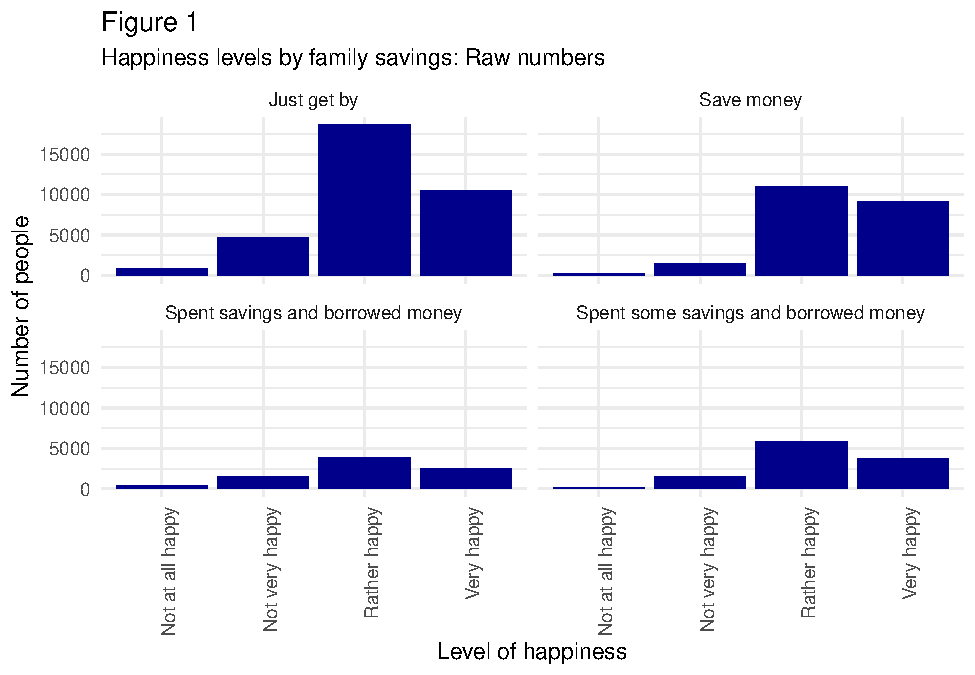
\includegraphics{610_final_files/figure-latex/happiness and family savings JW-1.pdf} 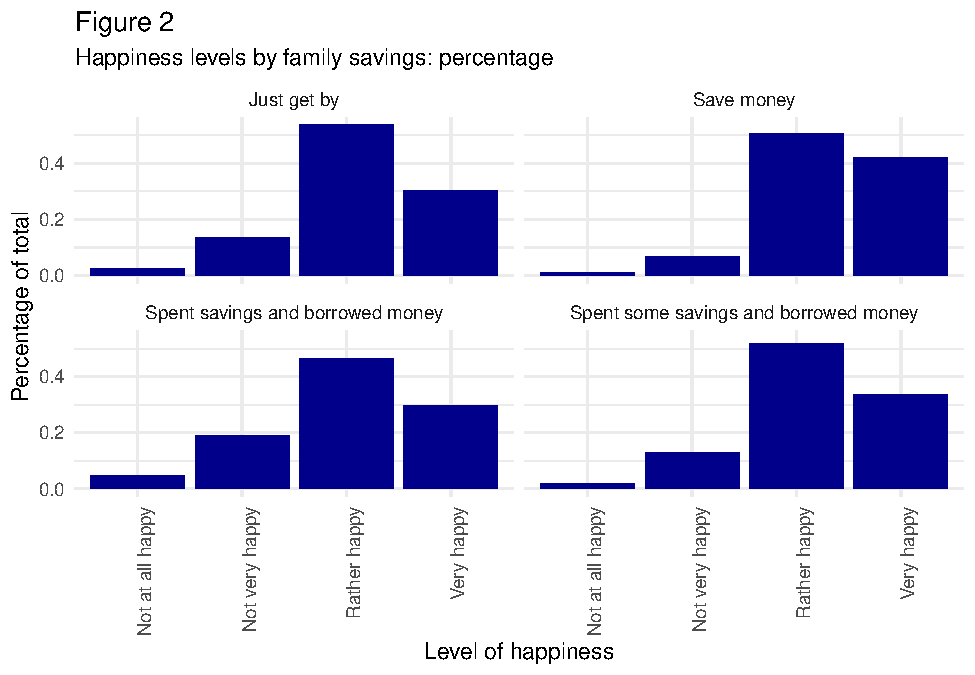
\includegraphics{610_final_files/figure-latex/happiness and family savings JW-2.pdf}

\begin{verbatim}
## # A tibble: 16 x 5
##    family_savings                   feeling_of_happine~     n total percent
##    <fct>                            <fct>               <int> <int>   <dbl>
##  1 Save money                       Not at all happy      203 21889 0.00927
##  2 Spent some savings and borrowed~ Not at all happy      207 11331 0.0183 
##  3 Just get by                      Not at all happy      813 34669 0.0235 
##  4 Spent savings and borrowed money Not at all happy      400  8333 0.0480 
##  5 Save money                       Not very happy       1449 21889 0.0662 
##  6 Spent some savings and borrowed~ Not very happy       1471 11331 0.130  
##  7 Just get by                      Not very happy       4650 34669 0.134  
##  8 Spent savings and borrowed money Not very happy       1577  8333 0.189  
##  9 Spent savings and borrowed money Very happy           2489  8333 0.299  
## 10 Just get by                      Very happy          10545 34669 0.304  
## 11 Spent some savings and borrowed~ Very happy           3800 11331 0.335  
## 12 Save money                       Very happy           9177 21889 0.419  
## 13 Spent savings and borrowed money Rather happy         3867  8333 0.464  
## 14 Save money                       Rather happy        11060 21889 0.505  
## 15 Spent some savings and borrowed~ Rather happy         5853 11331 0.517  
## 16 Just get by                      Rather happy        18661 34669 0.538
\end{verbatim}

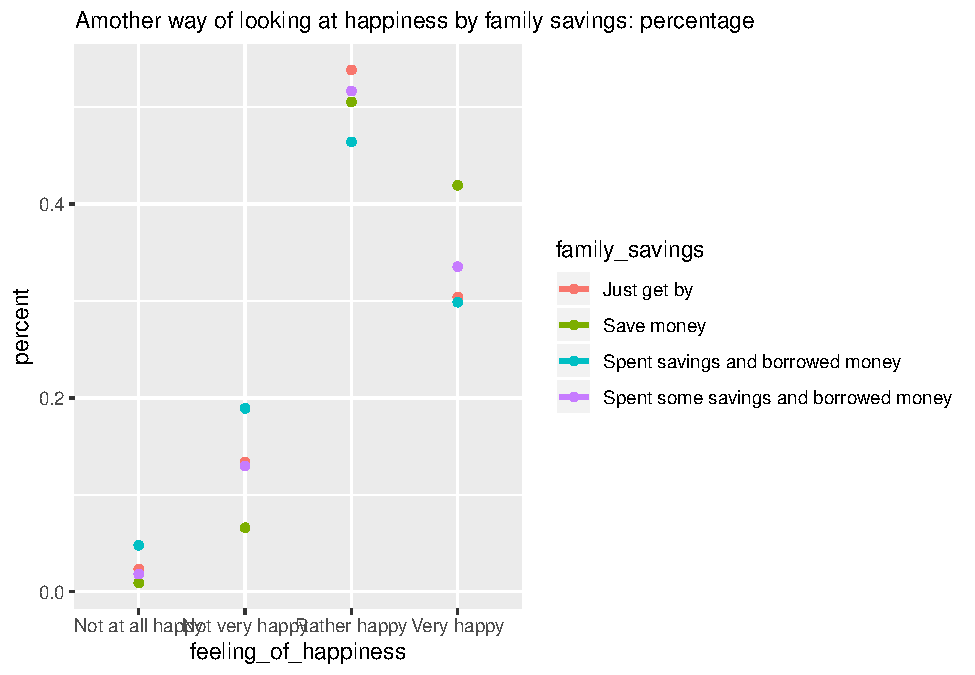
\includegraphics{610_final_files/figure-latex/happiness and family savings JW-3.pdf}

\begin{verbatim}
## List of 65
##  $ line                      :List of 6
##   ..$ colour       : chr "black"
##   ..$ size         : num 0.5
##   ..$ linetype     : num 1
##   ..$ lineend      : chr "butt"
##   ..$ arrow        : logi FALSE
##   ..$ inherit.blank: logi TRUE
##   ..- attr(*, "class")= chr [1:2] "element_line" "element"
##  $ rect                      :List of 5
##   ..$ fill         : chr "white"
##   ..$ colour       : chr "black"
##   ..$ size         : num 0.5
##   ..$ linetype     : num 1
##   ..$ inherit.blank: logi TRUE
##   ..- attr(*, "class")= chr [1:2] "element_rect" "element"
##  $ text                      :List of 11
##   ..$ family       : chr ""
##   ..$ face         : chr "plain"
##   ..$ colour       : chr "black"
##   ..$ size         : num 11
##   ..$ hjust        : num 0.5
##   ..$ vjust        : num 0.5
##   ..$ angle        : num 0
##   ..$ lineheight   : num 0.9
##   ..$ margin       : 'margin' num [1:4] 0pt 0pt 0pt 0pt
##   .. ..- attr(*, "valid.unit")= int 8
##   .. ..- attr(*, "unit")= chr "pt"
##   ..$ debug        : logi FALSE
##   ..$ inherit.blank: logi TRUE
##   ..- attr(*, "class")= chr [1:2] "element_text" "element"
##  $ axis.title.x              :List of 11
##   ..$ family       : NULL
##   ..$ face         : NULL
##   ..$ colour       : NULL
##   ..$ size         : NULL
##   ..$ hjust        : NULL
##   ..$ vjust        : num 1
##   ..$ angle        : NULL
##   ..$ lineheight   : NULL
##   ..$ margin       : 'margin' num [1:4] 2.75pt 0pt 0pt 0pt
##   .. ..- attr(*, "valid.unit")= int 8
##   .. ..- attr(*, "unit")= chr "pt"
##   ..$ debug        : NULL
##   ..$ inherit.blank: logi TRUE
##   ..- attr(*, "class")= chr [1:2] "element_text" "element"
##  $ axis.title.x.top          :List of 11
##   ..$ family       : NULL
##   ..$ face         : NULL
##   ..$ colour       : NULL
##   ..$ size         : NULL
##   ..$ hjust        : NULL
##   ..$ vjust        : num 0
##   ..$ angle        : NULL
##   ..$ lineheight   : NULL
##   ..$ margin       : 'margin' num [1:4] 0pt 0pt 2.75pt 0pt
##   .. ..- attr(*, "valid.unit")= int 8
##   .. ..- attr(*, "unit")= chr "pt"
##   ..$ debug        : NULL
##   ..$ inherit.blank: logi TRUE
##   ..- attr(*, "class")= chr [1:2] "element_text" "element"
##  $ axis.title.y              :List of 11
##   ..$ family       : NULL
##   ..$ face         : NULL
##   ..$ colour       : NULL
##   ..$ size         : NULL
##   ..$ hjust        : NULL
##   ..$ vjust        : num 1
##   ..$ angle        : num 90
##   ..$ lineheight   : NULL
##   ..$ margin       : 'margin' num [1:4] 0pt 2.75pt 0pt 0pt
##   .. ..- attr(*, "valid.unit")= int 8
##   .. ..- attr(*, "unit")= chr "pt"
##   ..$ debug        : NULL
##   ..$ inherit.blank: logi TRUE
##   ..- attr(*, "class")= chr [1:2] "element_text" "element"
##  $ axis.title.y.right        :List of 11
##   ..$ family       : NULL
##   ..$ face         : NULL
##   ..$ colour       : NULL
##   ..$ size         : NULL
##   ..$ hjust        : NULL
##   ..$ vjust        : num 0
##   ..$ angle        : num -90
##   ..$ lineheight   : NULL
##   ..$ margin       : 'margin' num [1:4] 0pt 0pt 0pt 2.75pt
##   .. ..- attr(*, "valid.unit")= int 8
##   .. ..- attr(*, "unit")= chr "pt"
##   ..$ debug        : NULL
##   ..$ inherit.blank: logi TRUE
##   ..- attr(*, "class")= chr [1:2] "element_text" "element"
##  $ axis.text                 :List of 11
##   ..$ family       : NULL
##   ..$ face         : NULL
##   ..$ colour       : chr "grey30"
##   ..$ size         : 'rel' num 0.8
##   ..$ hjust        : NULL
##   ..$ vjust        : NULL
##   ..$ angle        : NULL
##   ..$ lineheight   : NULL
##   ..$ margin       : NULL
##   ..$ debug        : NULL
##   ..$ inherit.blank: logi TRUE
##   ..- attr(*, "class")= chr [1:2] "element_text" "element"
##  $ axis.text.x               :List of 11
##   ..$ family       : NULL
##   ..$ face         : NULL
##   ..$ colour       : NULL
##   ..$ size         : NULL
##   ..$ hjust        : num 1
##   ..$ vjust        : num 1
##   ..$ angle        : num 90
##   ..$ lineheight   : NULL
##   ..$ margin       : 'margin' num [1:4] 2.2pt 0pt 0pt 0pt
##   .. ..- attr(*, "valid.unit")= int 8
##   .. ..- attr(*, "unit")= chr "pt"
##   ..$ debug        : NULL
##   ..$ inherit.blank: logi FALSE
##   ..- attr(*, "class")= chr [1:2] "element_text" "element"
##  $ axis.text.x.top           :List of 11
##   ..$ family       : NULL
##   ..$ face         : NULL
##   ..$ colour       : NULL
##   ..$ size         : NULL
##   ..$ hjust        : NULL
##   ..$ vjust        : num 0
##   ..$ angle        : NULL
##   ..$ lineheight   : NULL
##   ..$ margin       : 'margin' num [1:4] 0pt 0pt 2.2pt 0pt
##   .. ..- attr(*, "valid.unit")= int 8
##   .. ..- attr(*, "unit")= chr "pt"
##   ..$ debug        : NULL
##   ..$ inherit.blank: logi TRUE
##   ..- attr(*, "class")= chr [1:2] "element_text" "element"
##  $ axis.text.y               :List of 11
##   ..$ family       : NULL
##   ..$ face         : NULL
##   ..$ colour       : NULL
##   ..$ size         : NULL
##   ..$ hjust        : num 1
##   ..$ vjust        : NULL
##   ..$ angle        : NULL
##   ..$ lineheight   : NULL
##   ..$ margin       : 'margin' num [1:4] 0pt 2.2pt 0pt 0pt
##   .. ..- attr(*, "valid.unit")= int 8
##   .. ..- attr(*, "unit")= chr "pt"
##   ..$ debug        : NULL
##   ..$ inherit.blank: logi TRUE
##   ..- attr(*, "class")= chr [1:2] "element_text" "element"
##  $ axis.text.y.right         :List of 11
##   ..$ family       : NULL
##   ..$ face         : NULL
##   ..$ colour       : NULL
##   ..$ size         : NULL
##   ..$ hjust        : num 0
##   ..$ vjust        : NULL
##   ..$ angle        : NULL
##   ..$ lineheight   : NULL
##   ..$ margin       : 'margin' num [1:4] 0pt 0pt 0pt 2.2pt
##   .. ..- attr(*, "valid.unit")= int 8
##   .. ..- attr(*, "unit")= chr "pt"
##   ..$ debug        : NULL
##   ..$ inherit.blank: logi TRUE
##   ..- attr(*, "class")= chr [1:2] "element_text" "element"
##  $ axis.ticks                : list()
##   ..- attr(*, "class")= chr [1:2] "element_blank" "element"
##  $ axis.ticks.length         : 'unit' num 2.75pt
##   ..- attr(*, "valid.unit")= int 8
##   ..- attr(*, "unit")= chr "pt"
##  $ axis.ticks.length.x       : NULL
##  $ axis.ticks.length.x.top   : NULL
##  $ axis.ticks.length.x.bottom: NULL
##  $ axis.ticks.length.y       : NULL
##  $ axis.ticks.length.y.left  : NULL
##  $ axis.ticks.length.y.right : NULL
##  $ axis.line                 : list()
##   ..- attr(*, "class")= chr [1:2] "element_blank" "element"
##  $ axis.line.x               : NULL
##  $ axis.line.y               : NULL
##  $ legend.background         : list()
##   ..- attr(*, "class")= chr [1:2] "element_blank" "element"
##  $ legend.margin             : 'margin' num [1:4] 5.5pt 5.5pt 5.5pt 5.5pt
##   ..- attr(*, "valid.unit")= int 8
##   ..- attr(*, "unit")= chr "pt"
##  $ legend.spacing            : 'unit' num 11pt
##   ..- attr(*, "valid.unit")= int 8
##   ..- attr(*, "unit")= chr "pt"
##  $ legend.spacing.x          : NULL
##  $ legend.spacing.y          : NULL
##  $ legend.key                : list()
##   ..- attr(*, "class")= chr [1:2] "element_blank" "element"
##  $ legend.key.size           : 'unit' num 1.2lines
##   ..- attr(*, "valid.unit")= int 3
##   ..- attr(*, "unit")= chr "lines"
##  $ legend.key.height         : NULL
##  $ legend.key.width          : NULL
##  $ legend.text               :List of 11
##   ..$ family       : NULL
##   ..$ face         : NULL
##   ..$ colour       : NULL
##   ..$ size         : 'rel' num 0.8
##   ..$ hjust        : NULL
##   ..$ vjust        : NULL
##   ..$ angle        : NULL
##   ..$ lineheight   : NULL
##   ..$ margin       : NULL
##   ..$ debug        : NULL
##   ..$ inherit.blank: logi TRUE
##   ..- attr(*, "class")= chr [1:2] "element_text" "element"
##  $ legend.text.align         : NULL
##  $ legend.title              :List of 11
##   ..$ family       : NULL
##   ..$ face         : NULL
##   ..$ colour       : NULL
##   ..$ size         : NULL
##   ..$ hjust        : num 0
##   ..$ vjust        : NULL
##   ..$ angle        : NULL
##   ..$ lineheight   : NULL
##   ..$ margin       : NULL
##   ..$ debug        : NULL
##   ..$ inherit.blank: logi TRUE
##   ..- attr(*, "class")= chr [1:2] "element_text" "element"
##  $ legend.title.align        : NULL
##  $ legend.position           : chr "right"
##  $ legend.direction          : NULL
##  $ legend.justification      : chr "center"
##  $ legend.box                : NULL
##  $ legend.box.margin         : 'margin' num [1:4] 0cm 0cm 0cm 0cm
##   ..- attr(*, "valid.unit")= int 1
##   ..- attr(*, "unit")= chr "cm"
##  $ legend.box.background     : list()
##   ..- attr(*, "class")= chr [1:2] "element_blank" "element"
##  $ legend.box.spacing        : 'unit' num 11pt
##   ..- attr(*, "valid.unit")= int 8
##   ..- attr(*, "unit")= chr "pt"
##  $ panel.background          : list()
##   ..- attr(*, "class")= chr [1:2] "element_blank" "element"
##  $ panel.border              : list()
##   ..- attr(*, "class")= chr [1:2] "element_blank" "element"
##  $ panel.spacing             : 'unit' num 5.5pt
##   ..- attr(*, "valid.unit")= int 8
##   ..- attr(*, "unit")= chr "pt"
##  $ panel.spacing.x           : NULL
##  $ panel.spacing.y           : NULL
##  $ panel.grid                :List of 6
##   ..$ colour       : chr "grey92"
##   ..$ size         : NULL
##   ..$ linetype     : NULL
##   ..$ lineend      : NULL
##   ..$ arrow        : logi FALSE
##   ..$ inherit.blank: logi TRUE
##   ..- attr(*, "class")= chr [1:2] "element_line" "element"
##  $ panel.grid.minor          :List of 6
##   ..$ colour       : NULL
##   ..$ size         : 'rel' num 0.5
##   ..$ linetype     : NULL
##   ..$ lineend      : NULL
##   ..$ arrow        : logi FALSE
##   ..$ inherit.blank: logi TRUE
##   ..- attr(*, "class")= chr [1:2] "element_line" "element"
##  $ panel.ontop               : logi FALSE
##  $ plot.background           : list()
##   ..- attr(*, "class")= chr [1:2] "element_blank" "element"
##  $ plot.title                :List of 11
##   ..$ family       : NULL
##   ..$ face         : NULL
##   ..$ colour       : NULL
##   ..$ size         : 'rel' num 1.2
##   ..$ hjust        : num 0
##   ..$ vjust        : num 1
##   ..$ angle        : NULL
##   ..$ lineheight   : NULL
##   ..$ margin       : 'margin' num [1:4] 0pt 0pt 5.5pt 0pt
##   .. ..- attr(*, "valid.unit")= int 8
##   .. ..- attr(*, "unit")= chr "pt"
##   ..$ debug        : NULL
##   ..$ inherit.blank: logi TRUE
##   ..- attr(*, "class")= chr [1:2] "element_text" "element"
##  $ plot.subtitle             :List of 11
##   ..$ family       : NULL
##   ..$ face         : NULL
##   ..$ colour       : NULL
##   ..$ size         : NULL
##   ..$ hjust        : num 0
##   ..$ vjust        : num 1
##   ..$ angle        : NULL
##   ..$ lineheight   : NULL
##   ..$ margin       : 'margin' num [1:4] 0pt 0pt 5.5pt 0pt
##   .. ..- attr(*, "valid.unit")= int 8
##   .. ..- attr(*, "unit")= chr "pt"
##   ..$ debug        : NULL
##   ..$ inherit.blank: logi TRUE
##   ..- attr(*, "class")= chr [1:2] "element_text" "element"
##  $ plot.caption              :List of 11
##   ..$ family       : NULL
##   ..$ face         : NULL
##   ..$ colour       : NULL
##   ..$ size         : 'rel' num 0.8
##   ..$ hjust        : num 1
##   ..$ vjust        : num 1
##   ..$ angle        : NULL
##   ..$ lineheight   : NULL
##   ..$ margin       : 'margin' num [1:4] 5.5pt 0pt 0pt 0pt
##   .. ..- attr(*, "valid.unit")= int 8
##   .. ..- attr(*, "unit")= chr "pt"
##   ..$ debug        : NULL
##   ..$ inherit.blank: logi TRUE
##   ..- attr(*, "class")= chr [1:2] "element_text" "element"
##  $ plot.tag                  :List of 11
##   ..$ family       : NULL
##   ..$ face         : NULL
##   ..$ colour       : NULL
##   ..$ size         : 'rel' num 1.2
##   ..$ hjust        : num 0.5
##   ..$ vjust        : num 0.5
##   ..$ angle        : NULL
##   ..$ lineheight   : NULL
##   ..$ margin       : NULL
##   ..$ debug        : NULL
##   ..$ inherit.blank: logi TRUE
##   ..- attr(*, "class")= chr [1:2] "element_text" "element"
##  $ plot.tag.position         : chr "topleft"
##  $ plot.margin               : 'margin' num [1:4] 5.5pt 5.5pt 5.5pt 5.5pt
##   ..- attr(*, "valid.unit")= int 8
##   ..- attr(*, "unit")= chr "pt"
##  $ strip.background          : list()
##   ..- attr(*, "class")= chr [1:2] "element_blank" "element"
##  $ strip.placement           : chr "inside"
##  $ strip.text                :List of 11
##   ..$ family       : NULL
##   ..$ face         : NULL
##   ..$ colour       : chr "grey10"
##   ..$ size         : 'rel' num 0.8
##   ..$ hjust        : NULL
##   ..$ vjust        : NULL
##   ..$ angle        : NULL
##   ..$ lineheight   : NULL
##   ..$ margin       : 'margin' num [1:4] 4.4pt 4.4pt 4.4pt 4.4pt
##   .. ..- attr(*, "valid.unit")= int 8
##   .. ..- attr(*, "unit")= chr "pt"
##   ..$ debug        : NULL
##   ..$ inherit.blank: logi TRUE
##   ..- attr(*, "class")= chr [1:2] "element_text" "element"
##  $ strip.text.x              : NULL
##  $ strip.text.y              :List of 11
##   ..$ family       : NULL
##   ..$ face         : NULL
##   ..$ colour       : NULL
##   ..$ size         : NULL
##   ..$ hjust        : NULL
##   ..$ vjust        : NULL
##   ..$ angle        : num -90
##   ..$ lineheight   : NULL
##   ..$ margin       : NULL
##   ..$ debug        : NULL
##   ..$ inherit.blank: logi TRUE
##   ..- attr(*, "class")= chr [1:2] "element_text" "element"
##  $ strip.switch.pad.grid     : 'unit' num 2.75pt
##   ..- attr(*, "valid.unit")= int 8
##   ..- attr(*, "unit")= chr "pt"
##  $ strip.switch.pad.wrap     : 'unit' num 2.75pt
##   ..- attr(*, "valid.unit")= int 8
##   ..- attr(*, "unit")= chr "pt"
##  - attr(*, "class")= chr [1:2] "theme" "gg"
##  - attr(*, "complete")= logi TRUE
##  - attr(*, "validate")= logi TRUE
\end{verbatim}

As Figure 3 shows, although patterns of happiness levels are similar overall (e.g.~most people report being \enquote{Rather Happy}, fewest people report being \enquote{Not happy at all}), there are some differences of happiness level distributions between groups. A greater percentage of those with the lowest level of family savings (those who spent savings and borrowed money) reported being \enquote{Not at all happy} or \enquote{Not very happy}. On the other hand, the greatest percentage of people reporting being \enquote{Rather happy} were those who reported just getting by, and the greatest percentage of people reporting the highest level of happiness were those in the strongest financial position - those who saved money.

(NOTE: I'd like to use inline code here to reference exact percentages. How do put one cell value into inline code??)

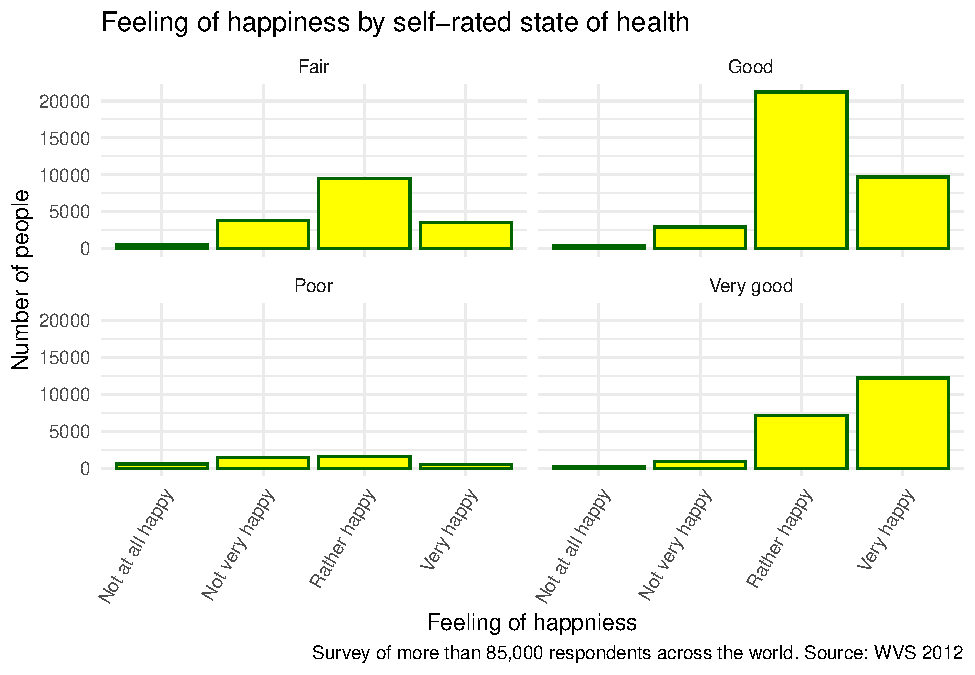
\includegraphics{610_final_files/figure-latex/trust and health-1.pdf}

\begin{tabular}{l|l|r}
\hline
most\_people\_trusted & feeling\_of\_happiness & n\\
\hline
Most people can be trusted & Not at all happy & 255\\
\hline
Most people can be trusted & Not very happy & 1528\\
\hline
Most people can be trusted & Rather happy & 10369\\
\hline
Most people can be trusted & Very happy & 6499\\
\hline
Need to be very careful & Not at all happy & 1368\\
\hline
Need to be very careful & Not very happy & 7619\\
\hline
Need to be very careful & Rather happy & 29072\\
\hline
Need to be very careful & Very happy & 19512\\
\hline
=======
Out of the total 76222 people, only slightly more than 24.47 percent say
they can trust most of the people around them, while 75.53 are caucious
about the society. Interstingly, there are more people feel happy in
life in the latter group than those in the former. Figure 1, below,
indicates such difference.

\begin{figure}
\centering
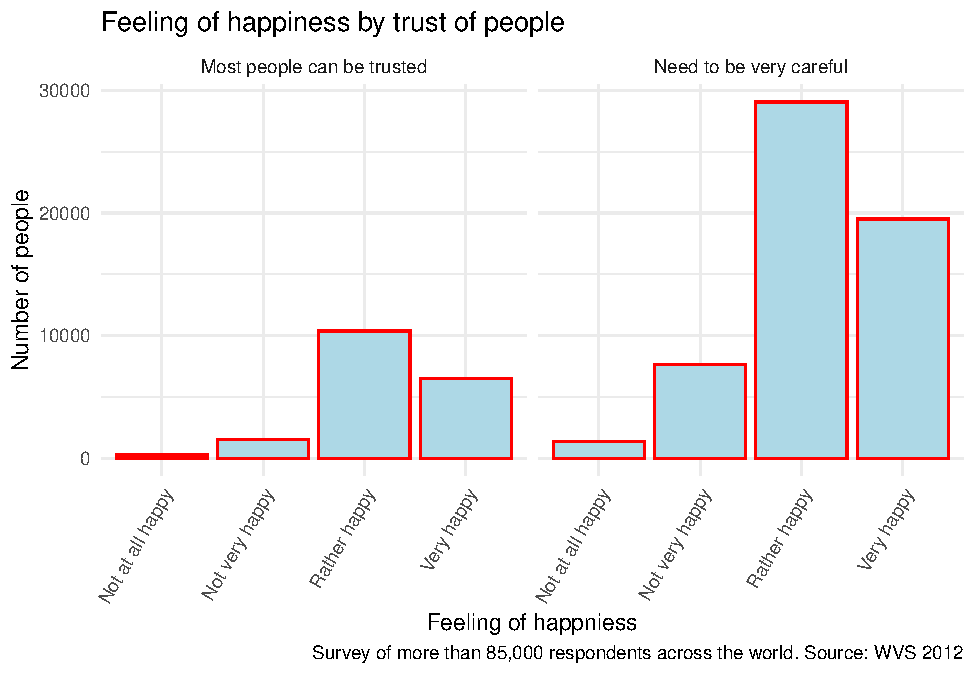
\includegraphics{610_final_files/figure-latex/unnamed-chunk-1-1.pdf}
\caption{}
\end{figure}

\subsubsection{Happiness and health
status}\label{happiness-and-health-status}

Our data suggest a positive correlation between health status and
perceived level of happiness. Figure 2, below, clearly indicates that
most of people who rated their health status as \enquote{good} also felt
happy.
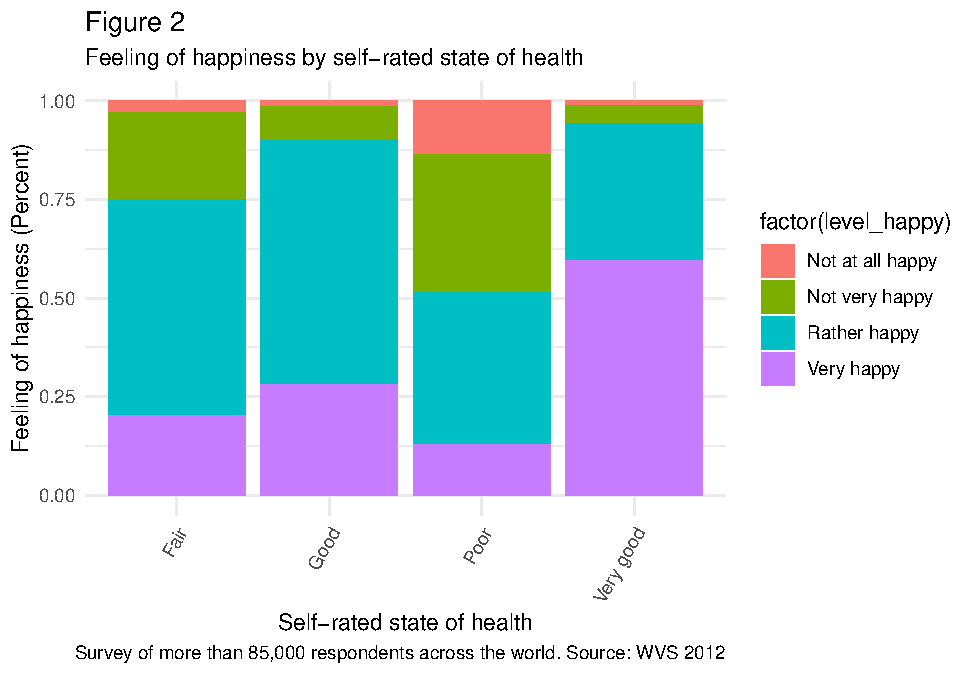
\includegraphics{610_final_files/figure-latex/unnamed-chunk-2-1.pdf}

\subsubsection{Happiness and family
savings}\label{happiness-and-family-savings}

Of the 76222 survey participants, the majority (45.48) reported just
getting by financially, while 28.72 saved money. The remainder spent
either some (14.87) or all (10.93) of their savings.

Table 1 shows happiness levels by level of family savings. Relationships
between happiness levels and family savings are explored in Figure 3.
Here, we see that of those reporting the lowest levels of happiness (Not
at all happy, Not very happy), most had spent all of their family
savings. On the other hand, of those reporting the highest level of
happiness (Very happy), the highest percentage were those in the
strongest financial position - those who saved money.

\begin{table}[tbp]
\begin{center}
\begin{threeparttable}
\caption{\label{tab:happiness by family APA table}}
\begin{tabular}{lllll}
\toprule
family\_savings & \multicolumn{1}{c}{feeling\_of\_happiness} & \multicolumn{1}{c}{n} & \multicolumn{1}{c}{total} & \multicolumn{1}{c}{percent}\\
\midrule
Just get by & Not at all happy & 813 & 34669 & 2.35\\
Just get by & Not very happy & 4650 & 34669 & 13.41\\
Just get by & Rather happy & 18661 & 34669 & 53.83\\
Just get by & Very happy & 10545 & 34669 & 30.42\\
Save money & Not at all happy & 203 & 21889 & 0.93\\
Save money & Not very happy & 1449 & 21889 & 6.62\\
Save money & Rather happy & 11060 & 21889 & 50.53\\
Save money & Very happy & 9177 & 21889 & 41.93\\
Spent savings and borrowed money & Not at all happy & 400 & 8333 & 4.80\\
Spent savings and borrowed money & Not very happy & 1577 & 8333 & 18.92\\
Spent savings and borrowed money & Rather happy & 3867 & 8333 & 46.41\\
Spent savings and borrowed money & Very happy & 2489 & 8333 & 29.87\\
Spent some savings and borrowed money & Not at all happy & 207 & 11331 & 1.83\\
Spent some savings and borrowed money & Not very happy & 1471 & 11331 & 12.98\\
Spent some savings and borrowed money & Rather happy & 5853 & 11331 & 51.65\\
Spent some savings and borrowed money & Very happy & 3800 & 11331 & 33.54\\
\bottomrule
>>>>>>> master
\end{tabular}
\end{threeparttable}
\end{center}
\end{table}

<<<<<<< HEAD
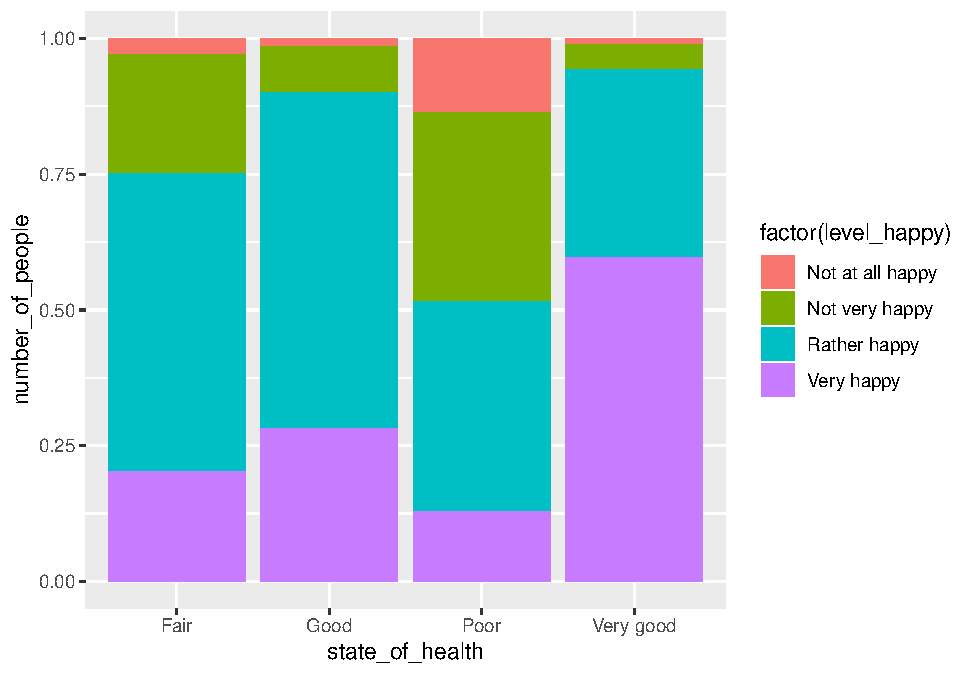
\includegraphics{610_final_files/figure-latex/trust and health-2.pdf}

\hypertarget{introduction}{%
\section{Introduction}\label{introduction}}

Study of happiness and its causal factors has been flourished in recent years. This project explores the relationship between happiness and some candidate variables, namely marital status, religious affiliation, level of income, status of heath, and level of trust. We use individual level survey of more than 85,000 respondents across 60 countries and societies around the world in World Value Survey Dataset 2012.

Scholars have studied the relationship between happines and political system (Inglehart, 2009)\ldots{}

Johnson (2012) finds that \enquote{trust as measured by the World Values Survey is positively correlated with experimentally measured trust}.

Gandelman and Hernández-Murillo (2013) reviews relationship of self-rate health status and perceived life quality.

Asha trying citation (Stack \& Eshleman, 1998)

\hypertarget{methods}{%
\section{Methods}\label{methods}}

We report how we determined our sample size, all data exclusions (if any), all manipulations, and all measures in the study.

\hypertarget{data-analysis}{%
\subsection{Data analysis}\label{data-analysis}}

\hypertarget{happiness-and-trust}{%
\subsubsection{Happiness and trust}\label{happiness-and-trust}}

Out of the total 76222 people, only slightly more than 24.47 percent say they can trust most of the people around them, while 75.53 is caucious about the society.

See below
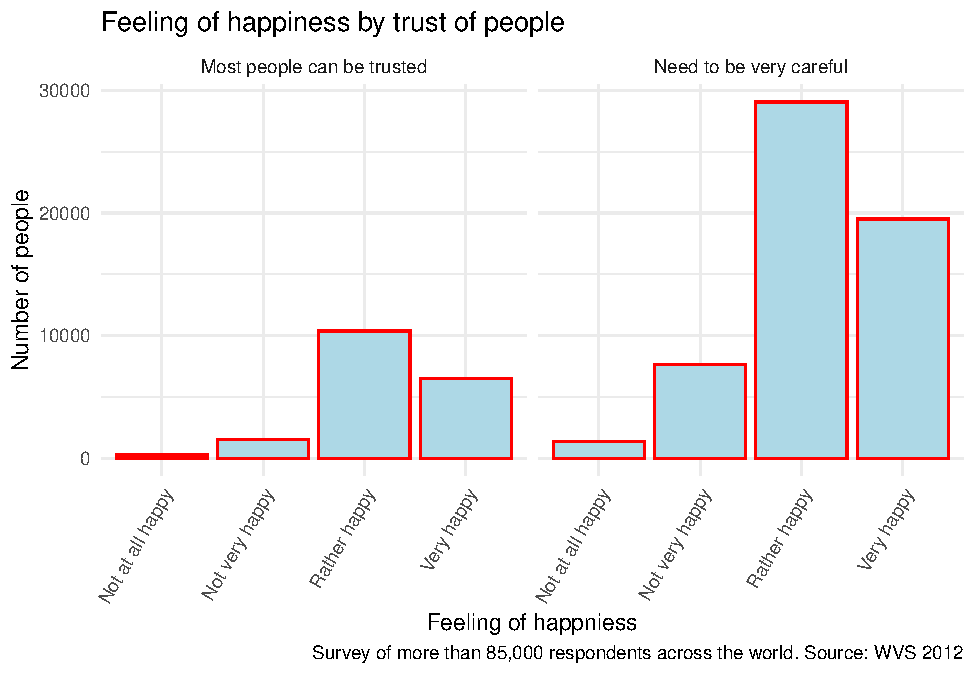
\includegraphics{610_final_files/figure-latex/unnamed-chunk-1-1.pdf}
it shows us
We used R (Version 3.6.1; R Core Team, 2018) and the R-packages \emph{dplyr} (Version 0.8.3; Wickham et al., 2019), \emph{forcats} (Version 0.4.0; Wickham, 2019a), \emph{ggplot2} (Version 3.2.1; Wickham, 2016), \emph{here} (Version 0.1; Müller, 2017), \emph{janitor} (Version 1.2.0; Firke, 2019), \emph{kableExtra} (Version 1.1.0; Zhu, 2019), \emph{knitr} (Version 1.25; Xie, 2015), \emph{papaja} (Version 0.1.0.9842; Aust \& Barth, 2018), \emph{purrr} (Version 0.3.3; Henry \& Wickham, 2019), \emph{readr} (Version 1.3.1; Wickham, Hester, \& Francois, 2018), \emph{rio} (Version 0.5.16; Chan, Chan, Leeper, \& Becker, 2018), \emph{stringr} (Version 1.4.0; Wickham, 2019b), \emph{tibble} (Version 2.1.3; Müller \& Wickham, 2019), \emph{tidyr} (Version 1.0.0; Wickham \& Henry, 2019), and \emph{tidyverse} (Version 1.2.1; Wickham, 2017) for all our analyses.

\hypertarget{results}{%
\section{Results}\label{results}}

\hypertarget{discussion}{%
\section{Discussion}\label{discussion}}
=======
\begin{figure}
\centering
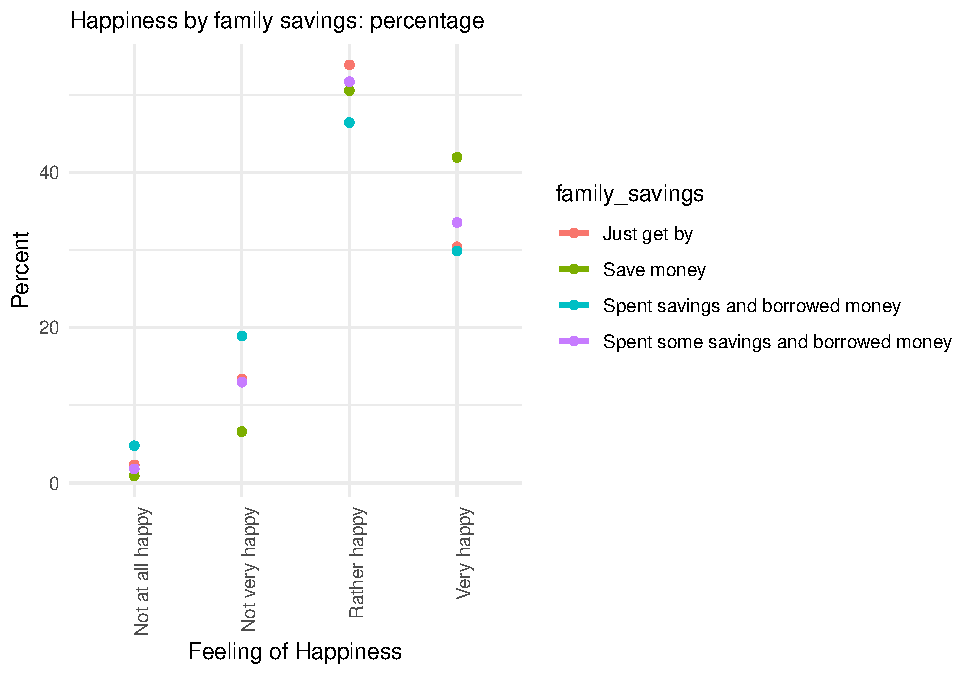
\includegraphics{610_final_files/figure-latex/happiness by family savings tables and figures-1.pdf}
\caption{}
\end{figure}

\section{Discussion}\label{discussion}
>>>>>>> master

Our results illuminate a number of connections between happiness levels
and other life factors such as trust of others, family financial status,
and health.

Data for happiness levels overall were normally distributed, with the
majority of participants reporting a moderate level of happiness, and
fewer reporting very low or very high levels of happiness. This pattern
continued to be evident when data were grouped by our independent
variables.

Contrary to the conventional belief that people who feel they can trust
people around them should feel more secured, hence happier. The data
shows us somewhat the opposite. Those who say they should be careful
with the fellows surrounding them indicates higher level of happiness.

Results indicate that good health is associated with greater feelings of
happiness. This affirms prior research by Gandelman and
Hernández-Murillo (2013) which found a strong relationship between
self-rated health status and perceived life quality.

Results also suggest a positive relationship between family financial
circumstances and happiness. Prior research has demonstrated a positive
association between income and well-being, although the mechanisms for
this remain unclear (Diener, 2010). Our results build on this work by
indicating that degree to which families are able to save money, or the
degree to which they must deplete savings and/or take out loans, are
areas worthy of further study.

Our results should be interpreted with caution. Because we are beginners
in using R, data analyses are, so far, only descriptive. Linear models
are needed to explore whether the relationships suggested here are
statistically significant. Furthermore, even if they were, these data
are cross-sectional, so findings cannot be interpreted as indicating
causality.

\newpage

\hypertarget{references}{%
\section{References}\label{references}}

\begingroup
\setlength{\parindent}{-0.5in}
\setlength{\leftskip}{0.5in}

\hypertarget{refs}{}
<<<<<<< HEAD
\leavevmode\hypertarget{ref-R-papaja}{}%
Aust, F., \& Barth, M. (2018). \emph{papaja: Create APA manuscripts with R Markdown}. Retrieved from \url{https://github.com/crsh/papaja}

\leavevmode\hypertarget{ref-R-rio}{}%
Chan, C.-h., Chan, G. C., Leeper, T. J., \& Becker, J. (2018). \emph{Rio: A swiss-army knife for data file i/o}.

\leavevmode\hypertarget{ref-R-janitor}{}%
Firke, S. (2019). \emph{Janitor: Simple tools for examining and cleaning dirty data}. Retrieved from \url{https://CRAN.R-project.org/package=janitor}

\leavevmode\hypertarget{ref-gandelman2013happiness}{}%
Gandelman, N., \& Hernández-Murillo, R. (2013). What do happiness and health satisfaction data tell us about relative risk aversion? \emph{Journal of Economic Psychology}, \emph{39}, 301--312.

\leavevmode\hypertarget{ref-R-purrr}{}%
Henry, L., \& Wickham, H. (2019). \emph{Purrr: Functional programming tools}. Retrieved from \url{https://CRAN.R-project.org/package=purrr}

\leavevmode\hypertarget{ref-inglehart200911}{}%
Inglehart, R. (2009). 11. Democracy and happiness: What causes what? \emph{Happiness, Economics and Politics: Towards a Multi-Disciplinary Approach}, 256.

\leavevmode\hypertarget{ref-johnson2012much}{}%
Johnson, N. D., \& Mislin, A. (2012). How much should we trust the world values survey trust question? \emph{Economics Letters}, \emph{116}(2), 210--212.

\leavevmode\hypertarget{ref-R-here}{}%
Müller, K. (2017). \emph{Here: A simpler way to find your files}. Retrieved from \url{https://CRAN.R-project.org/package=here}

\leavevmode\hypertarget{ref-R-tibble}{}%
Müller, K., \& Wickham, H. (2019). \emph{Tibble: Simple data frames}. Retrieved from \url{https://CRAN.R-project.org/package=tibble}

\leavevmode\hypertarget{ref-R-base}{}%
R Core Team. (2018). \emph{R: A language and environment for statistical computing}. Vienna, Austria: R Foundation for Statistical Computing. Retrieved from \url{https://www.R-project.org/}

\leavevmode\hypertarget{ref-stack1998marital}{}%
Stack, S., \& Eshleman, J. R. (1998). Marital status and happiness: A 17-nation study. \emph{Journal of Marriage and the Family}, 527--536.

\leavevmode\hypertarget{ref-R-ggplot2}{}%
Wickham, H. (2016). \emph{Ggplot2: Elegant graphics for data analysis}. Springer-Verlag New York. Retrieved from \url{https://ggplot2.tidyverse.org}

\leavevmode\hypertarget{ref-R-tidyverse}{}%
Wickham, H. (2017). \emph{Tidyverse: Easily install and load the 'tidyverse'}. Retrieved from \url{https://CRAN.R-project.org/package=tidyverse}

\leavevmode\hypertarget{ref-R-forcats}{}%
Wickham, H. (2019a). \emph{Forcats: Tools for working with categorical variables (factors)}. Retrieved from \url{https://CRAN.R-project.org/package=forcats}

\leavevmode\hypertarget{ref-R-stringr}{}%
Wickham, H. (2019b). \emph{Stringr: Simple, consistent wrappers for common string operations}. Retrieved from \url{https://CRAN.R-project.org/package=stringr}

\leavevmode\hypertarget{ref-R-dplyr}{}%
Wickham, H., François, R., Henry, L., \& Müller, K. (2019). \emph{Dplyr: A grammar of data manipulation}. Retrieved from \url{https://CRAN.R-project.org/package=dplyr}

\leavevmode\hypertarget{ref-R-tidyr}{}%
Wickham, H., \& Henry, L. (2019). \emph{Tidyr: Tidy messy data}. Retrieved from \url{https://CRAN.R-project.org/package=tidyr}

\leavevmode\hypertarget{ref-R-readr}{}%
Wickham, H., Hester, J., \& Francois, R. (2018). \emph{Readr: Read rectangular text data}. Retrieved from \url{https://CRAN.R-project.org/package=readr}

\leavevmode\hypertarget{ref-R-knitr}{}%
Xie, Y. (2015). \emph{Dynamic documents with R and knitr} (2nd ed.). Boca Raton, Florida: Chapman; Hall/CRC. Retrieved from \url{https://yihui.name/knitr/}

\leavevmode\hypertarget{ref-R-kableExtra}{}%
Zhu, H. (2019). \emph{KableExtra: Construct complex table with 'kable' and pipe syntax}. Retrieved from \url{https://CRAN.R-project.org/package=kableExtra}

\endgroup

Final Paper

The final project must:

\begin{enumerate}
\def\labelenumi{(\alph{enumi})}
\tightlist
\item
  be a reproducible and dynamic APA manuscript produced with R Markdown, via
  the \{papaja\} package and include references to the extant literature;
\item
  be housed on GitHub, with contributions from all authors obvious;
\item
  demonstrate moving data from its raw \enquote{messy} format to a tidy data format
  through the R Markdown file, but not in the final document;
\item
  include at least two exploratory data visualizations, and
\item
  include at least summary statistics of the data in tables, although fitted
  models of any sort are an added bonus (not literally, there are not extra points
  for fitting a model).
\end{enumerate}

\hypertarget{the-points-for-the-final-project-are-broken-down-as-follows}{%
\subsection{The points for the final project are broken down as follows:}\label{the-points-for-the-final-project-are-broken-down-as-follows}}

\hypertarget{writing-abstract-intro-methods-results-discussion-references}{%
\subsubsection{Writing (abstract, intro, methods, results, discussion, references)}\label{writing-abstract-intro-methods-results-discussion-references}}

\begin{itemize}
\tightlist
\item
  30 points(25\%) Document is fully reproducible and housed on GitHub
\item
  25 points (21\%) Demonstrate use of inline code
\item
  5 points (4\%) Demonstrate tidying messy data
\item
  30 points (25\%) Two data visualizations
\item
  20 points(10 points each) (17\%) Production of at least one table (of summary
  statistics or model results)
\item
  10 points (8\%)
\end{itemize}

=======
\hypertarget{ref-diener2010}{}
Diener, N., E. (2010). Wealth and happiness across the world: Material
prosperity predicts life evaluation, whereas psychosocial prosperity
predicts positive feeling. \emph{Journal of Personality and Social
Psychology}, \emph{99}(1), 52--61.

\hypertarget{ref-gandelman2013happiness}{}
Gandelman, N., \& Hernández-Murillo, R. (2013). What do happiness and
health satisfaction data tell us about relative risk aversion?
\emph{Journal of Economic Psychology}, \emph{39}, 301--312.

\hypertarget{ref-inglehart200911}{}
Inglehart, R. (2009). 11. democracy and happiness: What causes what?
\emph{Happiness, Economics and Politics: Towards a Multi-Disciplinary
Approach}, 256.

\hypertarget{ref-johnson2012much}{}
Johnson, N. D., \& Mislin, A. (2012). How much should we trust the world
values survey trust question? \emph{Economics Letters}, \emph{116}(2),
210--212.

\hypertarget{ref-schyns1998crossnational}{}
Schyns, P. (1998). Crossnational differences in happiness: Economic and
cultural factors explored. \emph{Social Indicators Research},
\emph{43}(1-2), 3--26.

\endgroup

>>>>>>> master

\end{document}
